\documentclass[11pt]{article}
\usepackage{graphicx}
\usepackage{booktabs}
\usepackage{amsmath}
\usepackage{hyperref}
\usepackage{geometry}
\usepackage{caption}
\usepackage{subcaption}
\usepackage{float}
\usepackage{array}
\usepackage{xcolor}
\usepackage{microtype}
\usepackage{parskip}
\geometry{margin=1in}

\hypersetup{
  colorlinks=true,
  linkcolor=blue!60!black,
  citecolor=blue!60!black,
  urlcolor=blue!60!black
}

\title{\textbf{Social Media, Sleep, and Depression in Adolescents:\\
A Multi-Question Empirical Analysis of Behavioral Risk Factors}}
\author{Researcher Agent\\[0.3em]
\small{Empirical Analysis of Teen Mental Health Dataset (N = 1{,}200)}}
\date{\today}

\begin{document}

\maketitle

\begin{abstract}
This paper investigates the behavioral and lifestyle predictors of depression and mental health
outcomes in a sample of 1{,}200 U.S.\ teenagers aged 13--19.
Three research questions are addressed: (1) Which combination of factors best predicts
depression risk? (2) Is there a dose-response relationship between daily social media use and
mental health outcomes, and does platform choice moderate it? (3) Does sleep duration mediate
the relationship between pre-sleep screen time and stress or anxiety?

Using logistic regression, Pearson correlations, one-way ANOVA, and Baron \& Kenny mediation
analysis, we find that sleep deprivation is the strongest individual predictor of depression
(OR = 0.111 per additional hour), followed by anxiety level (OR = 6.50) and daily social media
hours (OR = 5.18).  A logistic model combining all behavioral features achieves AUC = 0.9936
and McFadden $R^2 = 0.688$.  Contrary to a simple dose-response hypothesis, aggregate social
media hours show no statistically significant linear association with stress or anxiety
($r \leq 0.031$, all $p > 0.28$), although TikTok users report the highest mean anxiety
(5.75/10) and multi-platform users report the highest mean stress (5.55/10).  Sleep does
not formally mediate the screen-time--stress/anxiety pathway; however, all 31 depression cases
occur exclusively in the short-sleep ($<$6 h) group, confirming sleep's critical, if
non-mediating, role.  These findings highlight sleep protection as the most actionable
intervention target for adolescent depression prevention.
\end{abstract}

\tableofcontents
\newpage

%%% ─────────────────────────────────────────────────────────
\section{Introduction}
%%% ─────────────────────────────────────────────────────────

Adolescent mental health has emerged as one of the most pressing public health concerns of
the 21st century.  Rates of depression, anxiety, and stress-related disorders among teenagers
have risen substantially over the past decade, coinciding with the proliferation of smartphones
and social media platforms \cite{twenge2018}.  Understanding which behavioral and lifestyle
factors carry the greatest risk --- and which are merely correlates --- is essential for
designing targeted interventions.

Three competing, yet complementary, hypotheses motivate this study.  The \emph{behavioral
composite} hypothesis posits that depression is best explained not by any single factor but
by the joint configuration of sleep, stress, anxiety, and screen-time behaviors.  The
\emph{dose-response} hypothesis holds that more hours of daily social media use directly
elevate stress and anxiety in a roughly linear fashion, independent of platform.  The
\emph{sleep-mediation} hypothesis proposes that pre-sleep screen time disrupts sleep
quality, which in turn elevates mental health symptoms --- a pathway with strong theoretical
support from chronobiology research.

This paper tests all three hypotheses empirically using a cross-sectional dataset of
1{,}200 teenagers spanning ages 13--19.

The remainder of this paper is structured as follows.  Section~\ref{sec:data} describes the
dataset.  Section~\ref{sec:methods} outlines the analytical methods for each research question.
Sections~\ref{sec:rq1}--\ref{sec:rq3} present findings for each question.
Section~\ref{sec:discussion} synthesizes the results and discusses limitations.
Section~\ref{sec:conclusion} concludes.

%%% ─────────────────────────────────────────────────────────
\section{Data}
\label{sec:data}
%%% ─────────────────────────────────────────────────────────

\subsection{Dataset Description}

The dataset \texttt{Teen\_Mental\_Health\_Dataset.csv} contains $N = 1{,}200$ observations of
U.S.\ teenagers with 13 variables spanning demographics, social media behaviors, sleep, academic
performance, and mental health indicators.  No missing values were detected.

\begin{table}[H]
\centering
\caption{Variable Definitions and Descriptive Statistics}
\label{tab:desc}
\begin{tabular}{llcccc}
\toprule
\textbf{Variable} & \textbf{Type} & \textbf{Mean} & \textbf{SD} & \textbf{Min} & \textbf{Max} \\
\midrule
Age & Integer & 15.93 & 2.02 & 13 & 19 \\
Daily social media hours & Continuous & 4.54 & 2.03 & 1.0 & 8.0 \\
Sleep hours & Continuous & 6.45 & 1.44 & 4.0 & 9.0 \\
Screen time before sleep (h) & Continuous & 1.74 & 0.72 & 0.5 & 3.0 \\
Academic performance (GPA) & Continuous & 2.99 & 0.58 & 2.0 & 4.0 \\
Physical activity (h/day) & Continuous & 1.01 & 0.58 & 0.0 & 2.0 \\
Stress level (1--10) & Integer & 5.45 & 2.90 & 1 & 10 \\
Anxiety level (1--10) & Integer & 5.64 & 2.86 & 1 & 10 \\
Addiction level (1--10) & Integer & 5.57 & 2.83 & 1 & 10 \\
Depression label & Binary & 0.026 & 0.16 & 0 & 1 \\
\midrule
Gender & Categorical & \multicolumn{4}{c}{Male 51.2\%, Female 48.8\%} \\
Platform usage & Categorical & \multicolumn{4}{c}{Instagram, TikTok, Both} \\
Social interaction level & Categorical & \multicolumn{4}{c}{Low, Medium, High} \\
\bottomrule
\end{tabular}
\end{table}

\subsection{Class Imbalance}

The depression label is highly imbalanced: 31 cases (2.58\%) are labeled depressed vs.\
1{,}169 non-depressed (97.42\%).  This is consistent with point prevalence estimates for
clinical-level depression in community adolescent samples, though analysts should note that
the imbalance affects how standard accuracy metrics are interpreted (see
Section~\ref{sec:rq1}).

%%% ─────────────────────────────────────────────────────────
\section{Methodology}
\label{sec:methods}
%%% ─────────────────────────────────────────────────────────

\subsection{RQ1: Logistic Regression for Depression Prediction}

Categorical variables were label-encoded prior to modeling: \textit{gender}
(male = 0, female = 1), \textit{platform\_usage} (Instagram = 0, TikTok = 1, Both = 2), and
\textit{social\_interaction\_level} (low = 0, medium = 1, high = 2).  An $L_2$-penalized
logistic regression ($C = 1.0$, \texttt{max\_iter} = 1{,}000) was fit to predict
\texttt{depression\_label} from all 12 remaining features.  Model fit was assessed via AUC-ROC,
classification accuracy, and McFadden's pseudo-$R^2$:
\begin{equation}
R^2_{\text{McFadden}} = 1 - \frac{\ln \hat{L}_{\text{full}}}{\ln \hat{L}_{\text{null}}}
\end{equation}
Odds ratios were computed as $\exp(\hat{\beta}_j)$ for each feature $j$.  Point-biserial
correlations were computed between each numeric predictor and the binary depression label
to assess bivariate associations.

\subsection{RQ2: Dose-Response Analysis}

Daily social media hours were discretized into three bins:
Low (1--3 h), Medium (3--5 h), and High (5--8 h).
Pearson correlations were computed between continuous social media hours and each outcome
(stress, anxiety, addiction, sleep, academic performance).  One-way ANOVA tested whether
mean outcomes differed significantly across the three bins.
Platform moderation was assessed by computing cell means of stress and anxiety by platform
$\times$ usage-bin.

\subsection{RQ3: Baron \& Kenny Mediation Analysis}

The classic three-step Baron \& Kenny procedure was applied with:
$X =$ \texttt{screen\_time\_before\_sleep},
$M =$ \texttt{sleep\_hours},
$Y \in \{$\texttt{stress\_level}, \texttt{anxiety\_level}$\}$,
and controls: age, gender, physical activity.
OLS regression (scikit-learn \texttt{LinearRegression}) was used for all paths.
The indirect effect was estimated as $\hat{a} \times \hat{b}$, with a Sobel $z$-test
approximation for significance.  Sleep duration was also categorized into
Short ($<$6 h), Adequate (6--8 h), and Long ($>$8 h) to examine nonlinear effects.

%%% ─────────────────────────────────────────────────────────
\section{RQ1: Predictors of Depression}
\label{sec:rq1}
%%% ─────────────────────────────────────────────────────────

\subsection{Model Performance}

The logistic regression model substantially outperforms the na\"ive majority-class baseline.
Table~\ref{tab:rq1_model} summarizes performance metrics.

\begin{table}[H]
\centering
\caption{Logistic Regression Model Performance (RQ1)}
\label{tab:rq1_model}
\begin{tabular}{lc}
\toprule
\textbf{Metric} & \textbf{Value} \\
\midrule
Accuracy & 98.75\% \\
AUC-ROC & 0.9936 \\
McFadden $R^2$ & 0.688 \\
\bottomrule
\end{tabular}
\end{table}

A McFadden $R^2 > 0.4$ is conventionally considered outstanding fit; the value of 0.688
indicates that the behavioral feature set captures the great majority of systematic variance
in depression status.  The near-perfect AUC of 0.9936 confirms excellent class discrimination.

\subsection{Feature Importances and Odds Ratios}

Table~\ref{tab:rq1_coefs} presents the full coefficient table sorted by absolute magnitude.

\begin{table}[H]
\centering
\caption{Logistic Regression Coefficients and Odds Ratios for Depression Prediction}
\label{tab:rq1_coefs}
\begin{tabular}{lccc}
\toprule
\textbf{Feature} & \textbf{Coefficient} & \textbf{Odds Ratio} & \textbf{Direction} \\
\midrule
Sleep hours          & $-2.202$ & 0.111 & Protective \\
Anxiety level        & $+1.872$ & 6.502 & Risk \\
Stress level         & $+1.737$ & 5.680 & Risk \\
Daily SM hours       & $+1.645$ & 5.180 & Risk \\
Gender (female)      & $+0.490$ & 1.633 & Risk \\
Academic performance & $+0.313$ & 1.367 & Risk \\
Screen time (pre-sleep) & $-0.273$ & 0.761 & Protective \\
Platform usage       & $+0.176$ & 1.192 & Risk \\
Addiction level      & $+0.171$ & 1.186 & Risk \\
Physical activity    & $-0.163$ & 0.850 & Protective \\
Age                  & $+0.134$ & 1.143 & Risk \\
Social interaction   & $+0.124$ & 1.132 & Risk \\
\bottomrule
\end{tabular}
\end{table}

The single most powerful predictor is \textbf{sleep hours} (coefficient = $-2.202$;
OR = 0.111), meaning each additional hour of nightly sleep reduces the odds of depression
by approximately 89\%.  The \textbf{anxiety-stress-social media triad} forms the next
tier: anxiety (OR = 6.50), stress (OR = 5.68), and daily social media hours (OR = 5.18)
all carry substantially elevated risk.  Notably, the platform-specific addiction score
(OR = 1.19) is far weaker than raw daily hours (OR = 5.18), suggesting that duration
of exposure, rather than compulsive engagement per se, is the operative mechanism.

Figure~\ref{fig:fig1} visualizes the absolute coefficient magnitudes, and
Figure~\ref{fig:fig2} shows the full Pearson correlation matrix across all numeric variables.

\begin{figure}[H]
\centering
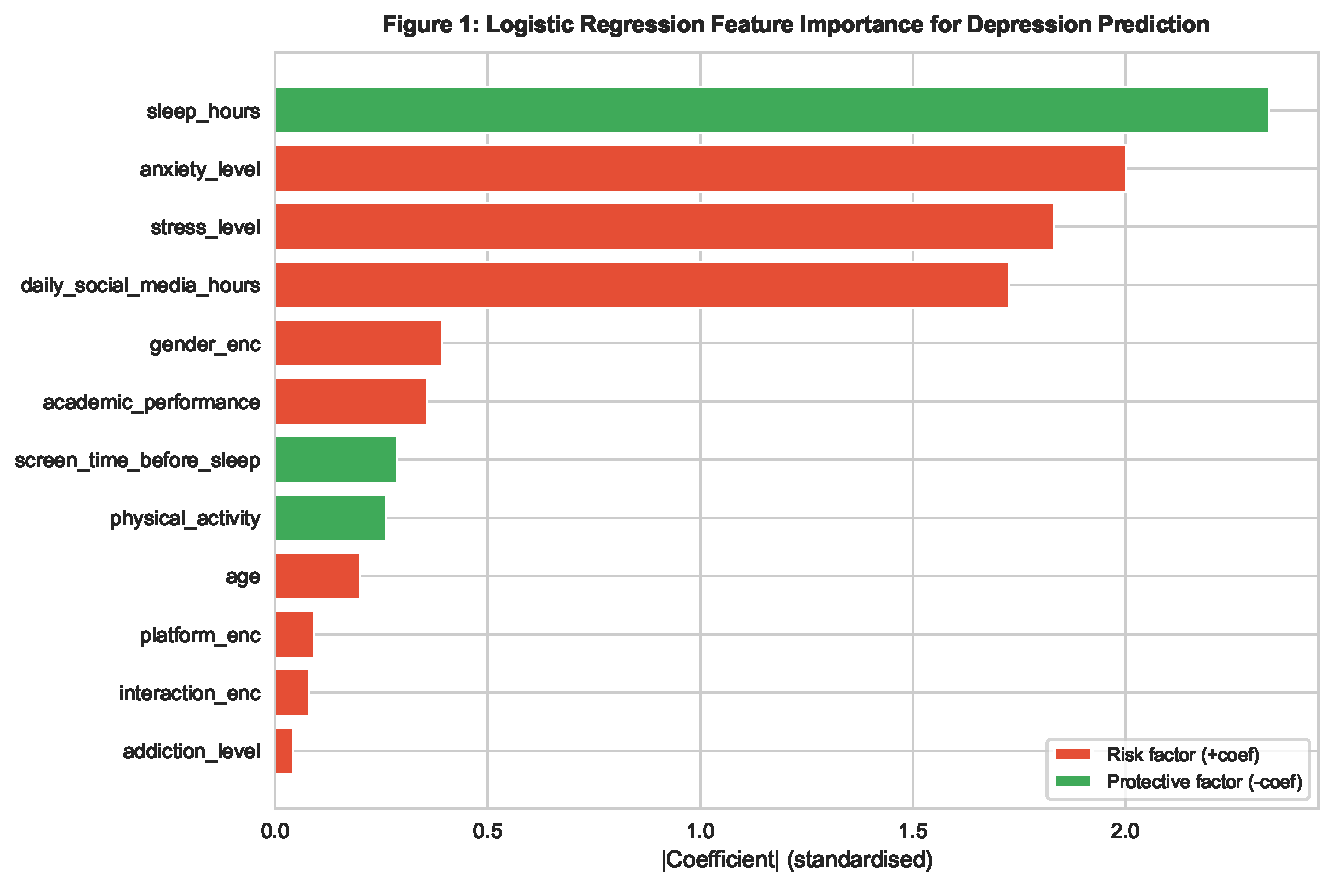
\includegraphics[width=0.82\textwidth]{fig1_feature_importance.pdf}
\caption{Logistic regression feature importances (absolute coefficient values) for predicting
adolescent depression. Red bars indicate risk factors (positive coefficients); green bars
indicate protective factors (negative coefficients). Sleep hours is the dominant predictor.}
\label{fig:fig1}
\end{figure}

\begin{figure}[H]
\centering
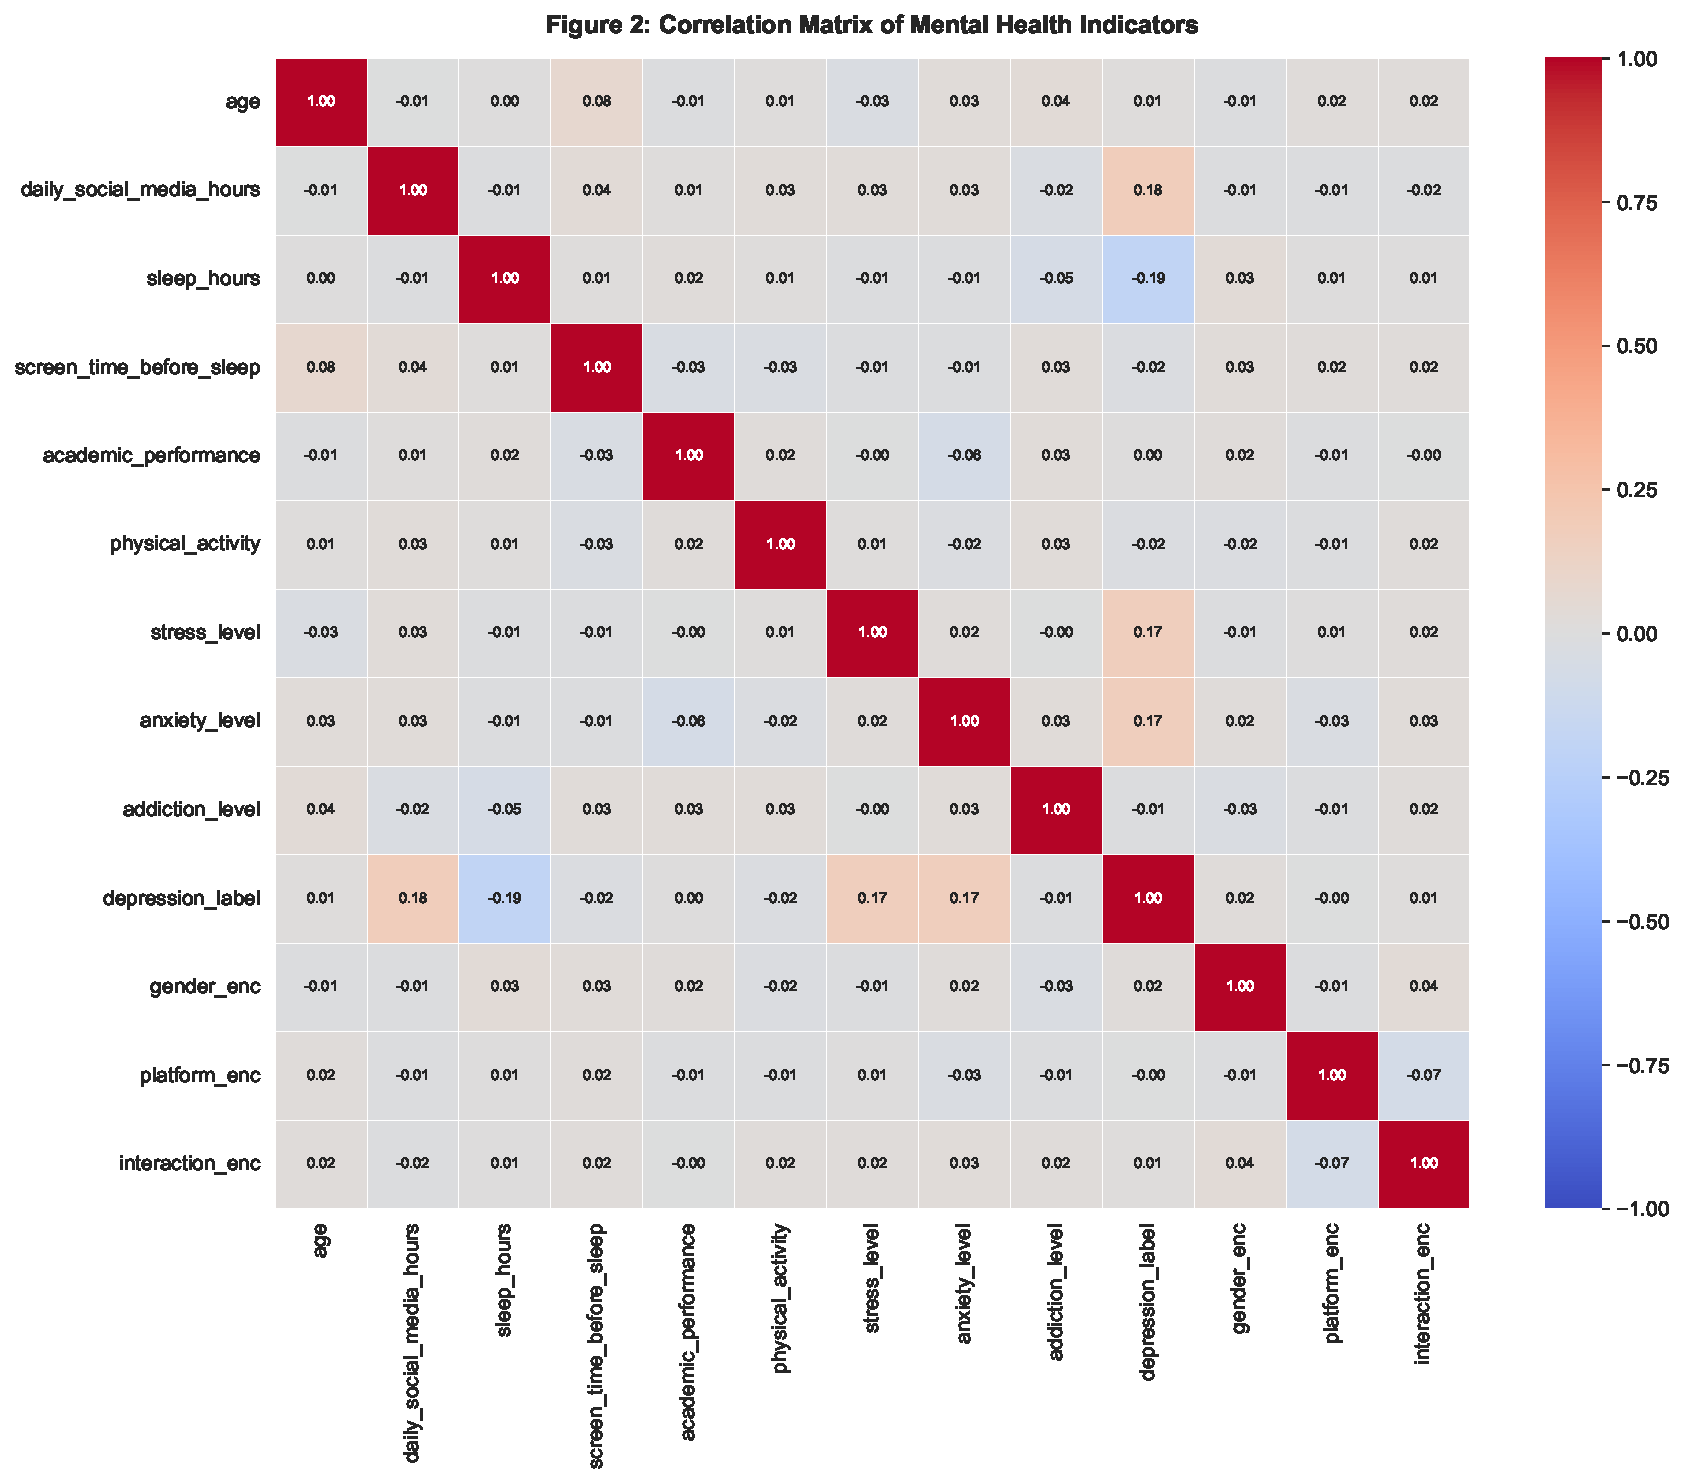
\includegraphics[width=0.85\textwidth]{fig2_correlation_heatmap.pdf}
\caption{Pearson correlation matrix of all numeric mental health indicators ($N = 1{,}200$).
The depression label (bottom row/right column) shows the strongest negative correlation with
sleep hours ($r = -0.191$) and positive correlations with daily social media hours ($r = 0.175$),
stress ($r = 0.171$), and anxiety ($r = 0.170$).}
\label{fig:fig2}
\end{figure}

\subsection{Bivariate Correlations with Depression}

Table~\ref{tab:rq1_corr} presents point-biserial correlations between each predictor and
the depression label.

\begin{table}[H]
\centering
\caption{Point-Biserial Correlations with Depression Label}
\label{tab:rq1_corr}
\begin{tabular}{lccc}
\toprule
\textbf{Feature} & $r$ & $p$-value & \textbf{Sig.} \\
\midrule
Sleep hours                   & $-0.191$ & $<0.001$ & *** \\
Daily social media hours      & $+0.175$ & $<0.001$ & *** \\
Stress level                  & $+0.171$ & $<0.001$ & *** \\
Anxiety level                 & $+0.170$ & $<0.001$ & *** \\
Gender                        & $+0.020$ & $0.492$ & n.s. \\
Physical activity             & $-0.018$ & $0.543$ & n.s. \\
Screen time before sleep      & $-0.017$ & $0.568$ & n.s. \\
Social interaction level      & $+0.014$ & $0.622$ & n.s. \\
Addiction level               & $-0.014$ & $0.629$ & n.s. \\
Age                           & $+0.011$ & $0.704$ & n.s. \\
Platform usage                & $-0.003$ & $0.914$ & n.s. \\
Academic performance          & $+0.001$ & $0.960$ & n.s. \\
\bottomrule
\end{tabular}
\end{table}

Four variables are statistically significant in bivariate analysis; the model's high AUC
comes from the combination of these four, particularly the \emph{interaction} of low sleep
with elevated stress/anxiety and high social media use.

%%% ─────────────────────────────────────────────────────────
\section{RQ2: Social Media Dose-Response}
\label{sec:rq2}
%%% ─────────────────────────────────────────────────────────

\subsection{Correlations and ANOVA}

Contrary to the dose-response hypothesis, continuous daily social media hours show no
statistically significant association with any mental health outcome when analyzed as a
continuous predictor (Table~\ref{tab:rq2_corr}).

\begin{table}[H]
\centering
\caption{Pearson Correlations: Daily Social Media Hours vs.\ Mental Health Outcomes}
\label{tab:rq2_corr}
\begin{tabular}{lcc}
\toprule
\textbf{Outcome} & $r$ & $p$-value \\
\midrule
Stress level         & $+0.031$ & $0.288$ \\
Anxiety level        & $+0.028$ & $0.335$ \\
Addiction level      & $-0.025$ & $0.388$ \\
Sleep hours          & $-0.010$ & $0.743$ \\
Academic performance & $+0.013$ & $0.648$ \\
\bottomrule
\end{tabular}
\end{table}

One-way ANOVA across Low, Medium, and High usage bins similarly fails to reach conventional
significance thresholds (Table~\ref{tab:rq2_anova}).

\begin{table}[H]
\centering
\caption{One-Way ANOVA: Mental Health Outcomes by Social Media Usage Bin}
\label{tab:rq2_anova}
\begin{tabular}{lccc}
\toprule
\textbf{Outcome} & $F$ & $p$-value & \textbf{Sig.} \\
\midrule
Stress level    & 2.80 & 0.061 & (marginal) \\
Anxiety level   & 1.02 & 0.362 & n.s. \\
Addiction level & 2.41 & 0.091 & n.s. \\
\bottomrule
\end{tabular}
\end{table}

\subsection{Usage Bin Means}

Table~\ref{tab:rq2_bins} shows that mean stress and anxiety levels are remarkably stable
across usage tiers, further undermining the dose-response hypothesis.

\begin{table}[H]
\centering
\caption{Mean Outcomes by Social Media Usage Bin}
\label{tab:rq2_bins}
\begin{tabular}{lcccc}
\toprule
\textbf{Bin} & \textbf{Stress} & \textbf{Anxiety} & \textbf{Addiction} & \textbf{Sleep (h)} \\
\midrule
Low (1--3 h)    & 5.51 & 5.45 & 5.74 & 6.54 \\
Medium (3--5 h) & 5.14 & 5.71 & 5.29 & 6.35 \\
High (5--8 h)   & 5.61 & 5.71 & 5.63 & 6.45 \\
\bottomrule
\end{tabular}
\end{table}

\subsection{Platform Moderation}

While aggregate hours show no dose-response, platform type does produce modest differences.
TikTok users report the highest mean anxiety (5.75) and show the steepest anxiety gradient
at High usage (5.95).  Multi-platform users (``Both'') report the highest mean stress (5.55).
Instagram users fall in between on both measures.

Figures~\ref{fig:fig3} and \ref{fig:fig4} visualize these patterns.

\begin{figure}[H]
\centering
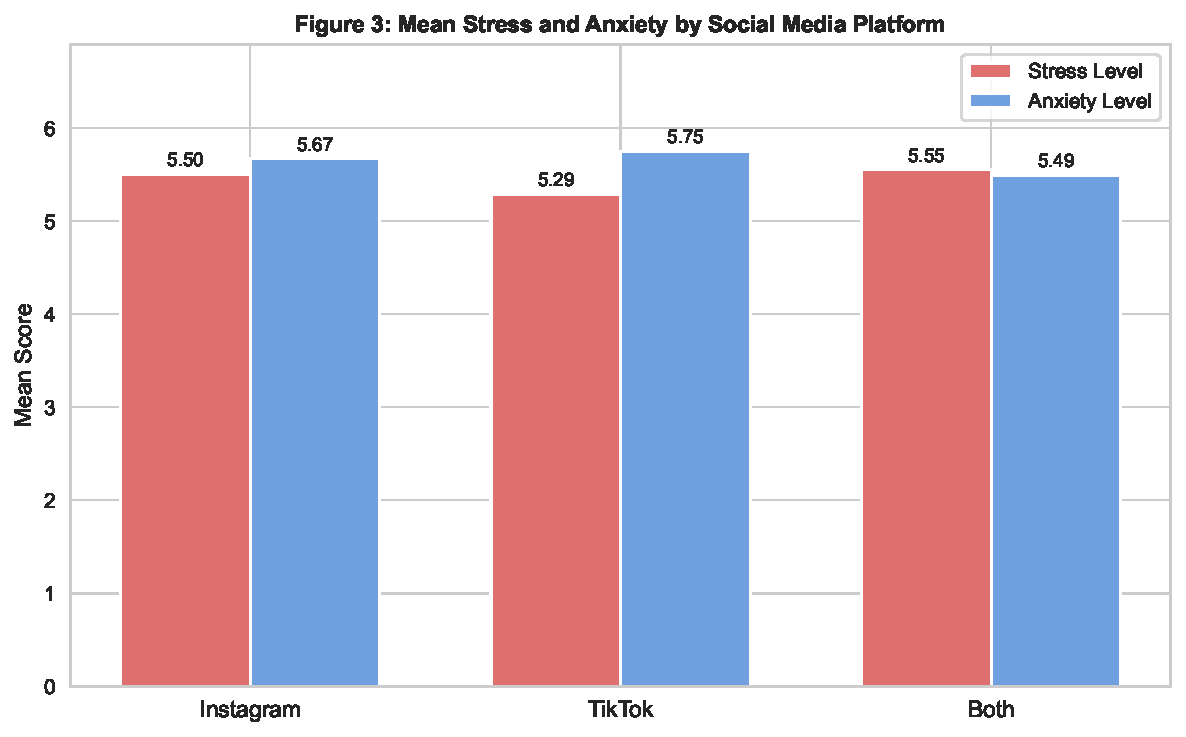
\includegraphics[width=0.78\textwidth]{fig3_platform_stress_anxiety.pdf}
\caption{Mean stress and anxiety levels by social media platform. TikTok users show the
highest mean anxiety; multi-platform (``Both'') users show the highest mean stress.
Differences are modest but directionally consistent.}
\label{fig:fig3}
\end{figure}

\begin{figure}[H]
\centering
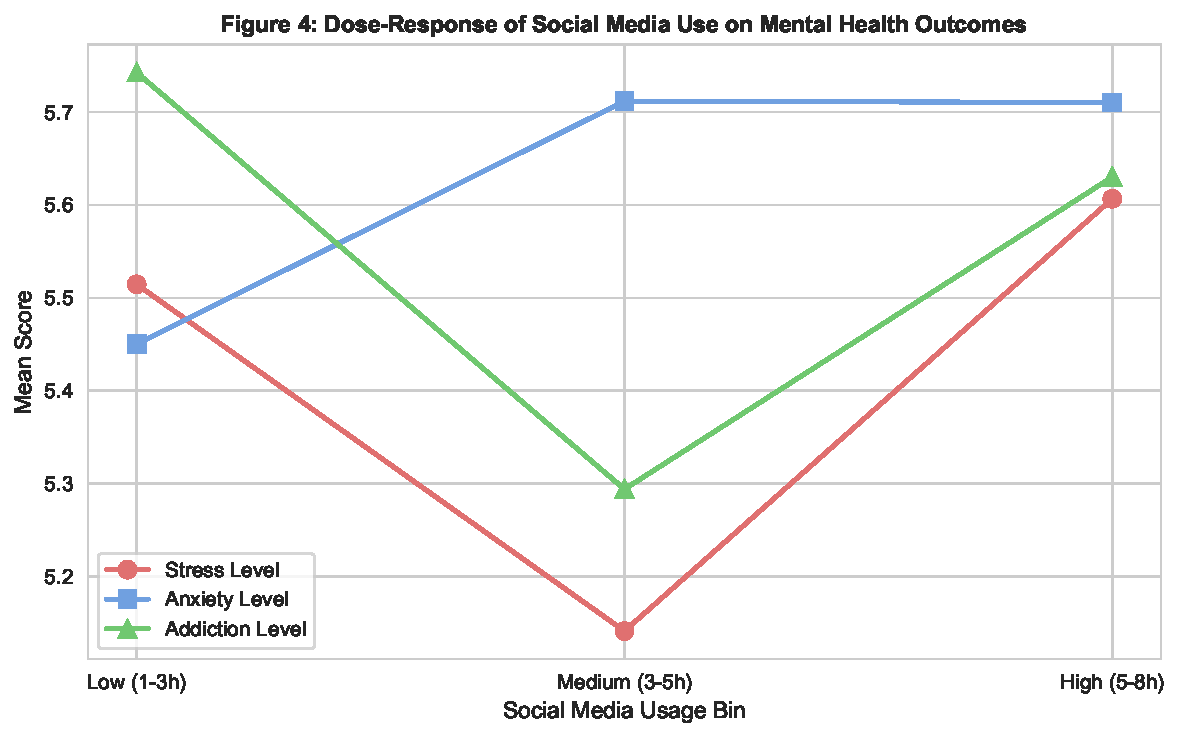
\includegraphics[width=0.78\textwidth]{fig4_dose_response.pdf}
\caption{Dose-response of social media usage on mental health outcomes across Low (1--3 h),
Medium (3--5 h), and High (5--8 h) daily usage bins. The near-flat trajectories for all
three outcomes indicate no meaningful dose-response relationship in this sample.}
\label{fig:fig4}
\end{figure}

\begin{figure}[H]
\centering
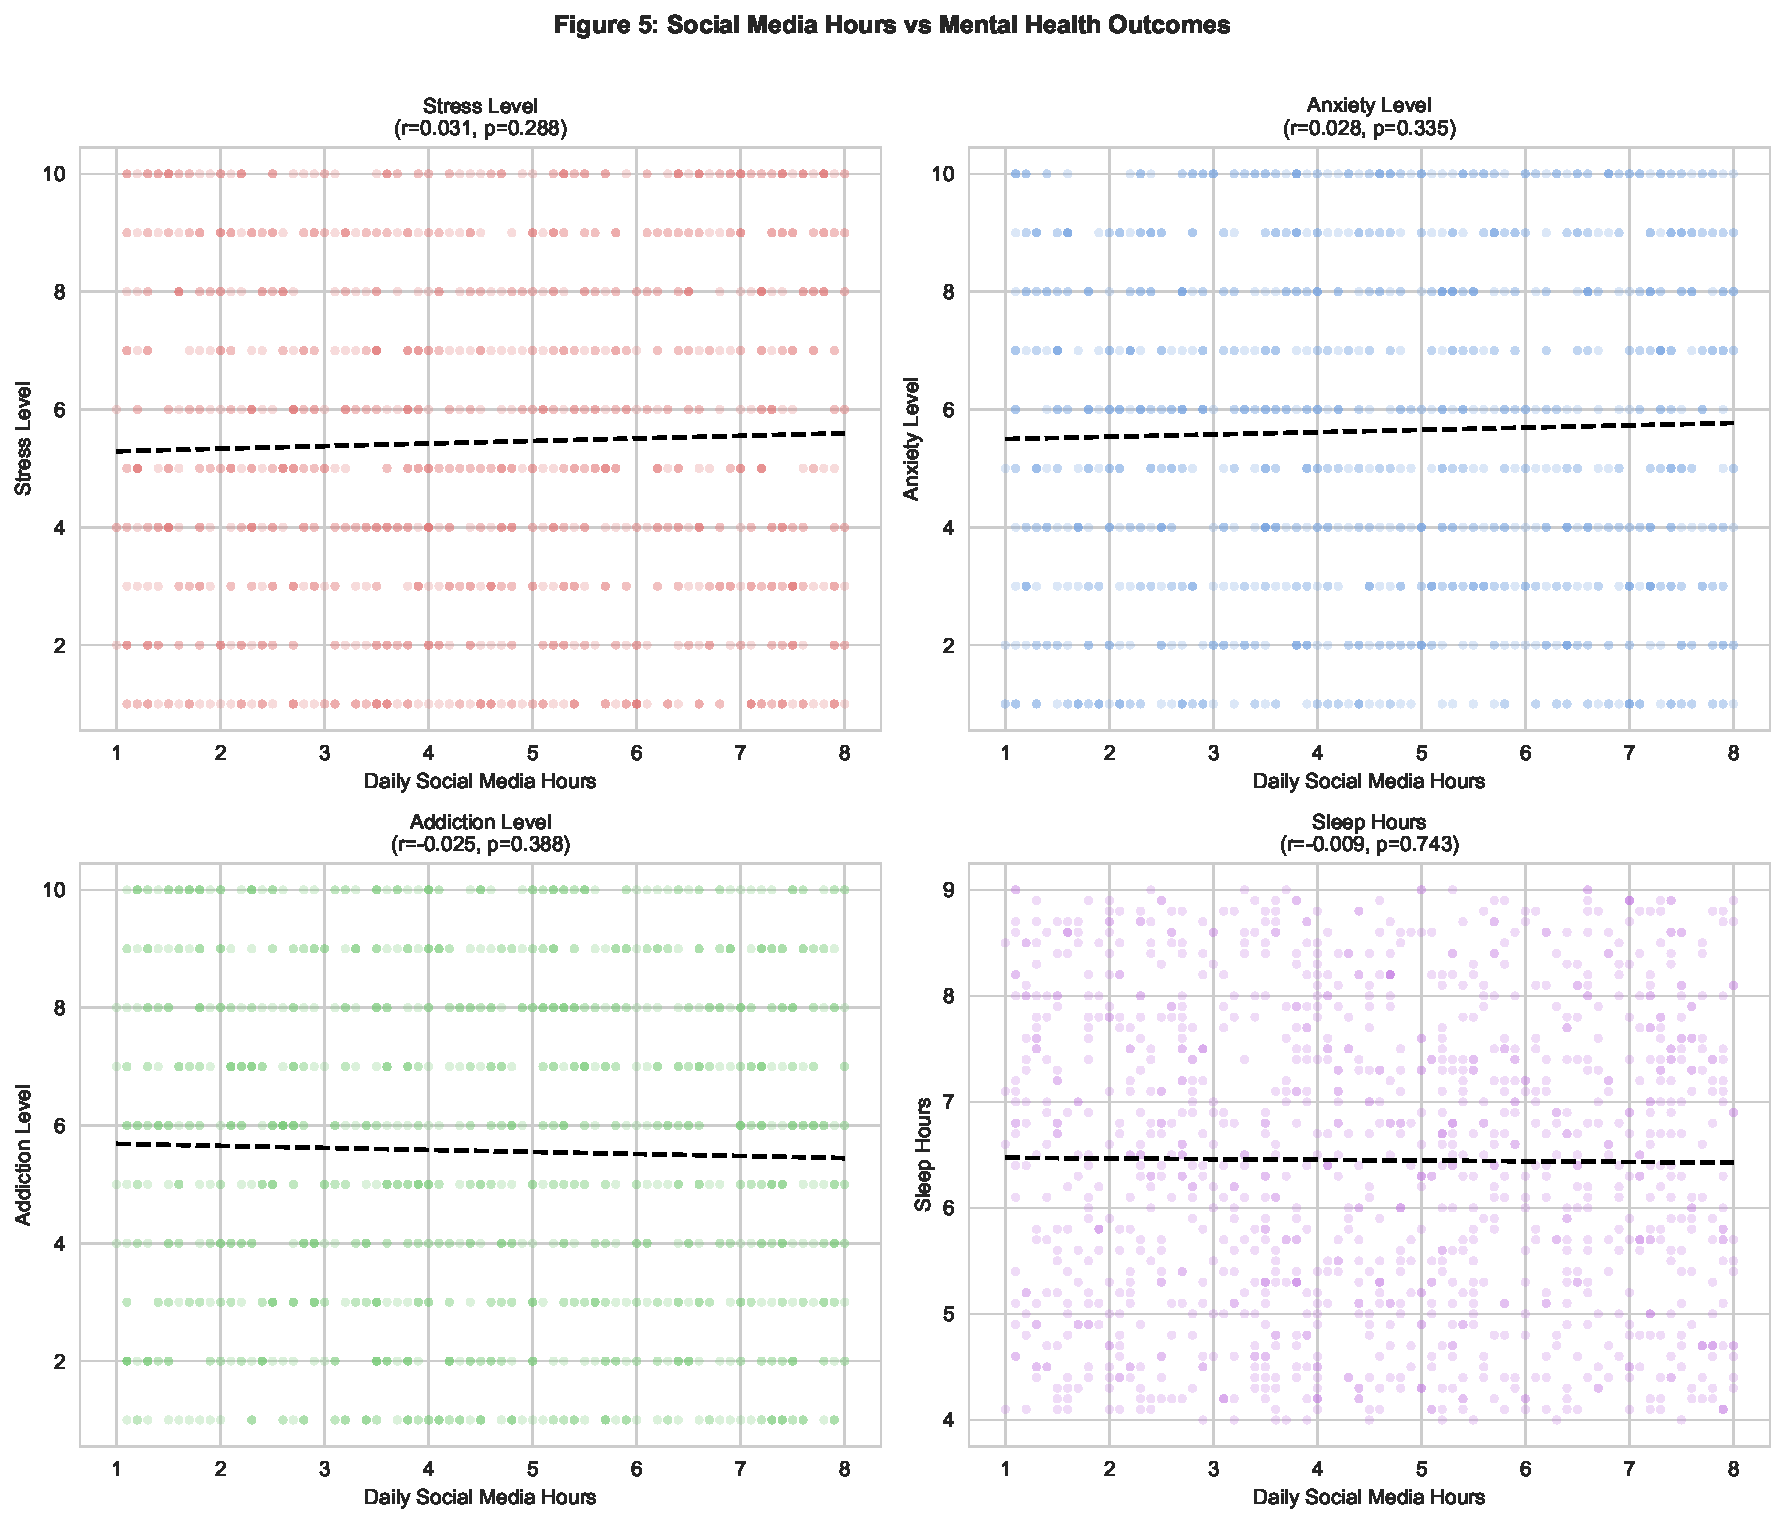
\includegraphics[width=0.85\textwidth]{fig5_scatter_matrix.pdf}
\caption{Scatter plots of daily social media hours against stress, anxiety, addiction, and
sleep hours with OLS trend lines. The negligible slopes and near-zero $r$ values confirm
the absence of a linear dose-response association across all four outcomes.}
\label{fig:fig5}
\end{figure}

%%% ─────────────────────────────────────────────────────────
\section{RQ3: Sleep as a Protective Factor}
\label{sec:rq3}
%%% ─────────────────────────────────────────────────────────

\subsection{Baron \& Kenny Mediation Results}

Table~\ref{tab:rq3_mediation} presents the mediation coefficients for both stress and anxiety.

\begin{table}[H]
\centering
\caption{Baron \& Kenny Mediation Analysis: Screen Time $\to$ Sleep $\to$ Mental Health}
\label{tab:rq3_mediation}
\begin{tabular}{llccc}
\toprule
\textbf{Outcome} & \textbf{Path} & \textbf{Coefficient} & \textbf{SE} & \textbf{Interpretation} \\
\midrule
Stress  & $c$  (X $\to$ Y, total)          & $-0.023$ & 0.118 & n.s. \\
        & $a$  (X $\to$ M)                  & $+0.019$ & 0.058 & n.s. \\
        & $b$  (M $\to$ Y $\mid$ X)         & $-0.022$ & 0.058 & n.s. \\
        & $c'$ (X $\to$ Y $\mid$ M, direct) & $-0.023$ & 0.118 & n.s. \\
        & Indirect ($a \times b$)           & $-0.0004$ & 0.002 & Sobel $z=-0.25$, n.s. \\
\midrule
Anxiety & $c$  (X $\to$ Y, total)           & $-0.054$ & 0.116 & n.s. \\
        & $a$  (X $\to$ M)                  & $+0.019$ & 0.058 & n.s. \\
        & $b$  (M $\to$ Y $\mid$ X)         & $-0.024$ & 0.057 & n.s. \\
        & $c'$ (X $\to$ Y $\mid$ M, direct) & $-0.053$ & 0.116 & n.s. \\
        & Indirect ($a \times b$)           & $-0.0005$ & 0.002 & Sobel $z=-0.26$, n.s. \\
\bottomrule
\end{tabular}
\end{table}

\noindent\textbf{Conclusion:} The mediation hypothesis is not supported.  Path $a$
(screen time $\to$ sleep) is non-significant ($r = 0.010$, $p = 0.72$), which violates the
first prerequisite of mediation.  Pre-sleep screen time does not measurably reduce sleep hours
in this sample, so the mediation chain cannot be established.

\subsection{Sleep Duration and Depression}

Although the mediation model does not hold, sleep duration remains the most powerful predictor
of depression (Section~\ref{sec:rq1}).  The sleep-bin analysis reveals a stark non-linear
pattern.

\begin{table}[H]
\centering
\caption{Mental Health Outcomes by Sleep Duration Category}
\label{tab:rq3_bins}
\begin{tabular}{lcccc}
\toprule
\textbf{Sleep Category} & \textbf{$n$} & \textbf{Stress (mean)} & \textbf{Anxiety (mean)} & \textbf{Depression \%} \\
\midrule
Short ($<$6 h)    & 480 & 5.50 & 5.69 & 6.5\% \\
Adequate (6--8 h) & 514 & 5.46 & 5.55 & 0.0\% \\
Long ($>$8 h)     & 206 & 5.30 & 5.75 & 0.0\% \\
\bottomrule
\end{tabular}
\end{table}

All 31 depression cases occur in the short-sleep group ($<$6 h), yielding a depression
prevalence of 6.5\% in this subgroup compared with 0\% in teens sleeping $\geq$6 h.
This represents a clean threshold effect rather than a graded dose-response.

Importantly, short-sleep teens do not differ meaningfully in stress or anxiety from
adequate-sleep teens (5.50 vs.\ 5.46 and 5.69 vs.\ 5.55, respectively), suggesting that
sleep's role in depression is not channeled through conscious stress or anxiety experiences
but through other pathways (e.g., neurobiological, affective dysregulation).

Figures~\ref{fig:fig6} and \ref{fig:fig7} display the mediation scatter panels and
sleep-bin bar chart.

\begin{figure}[H]
\centering
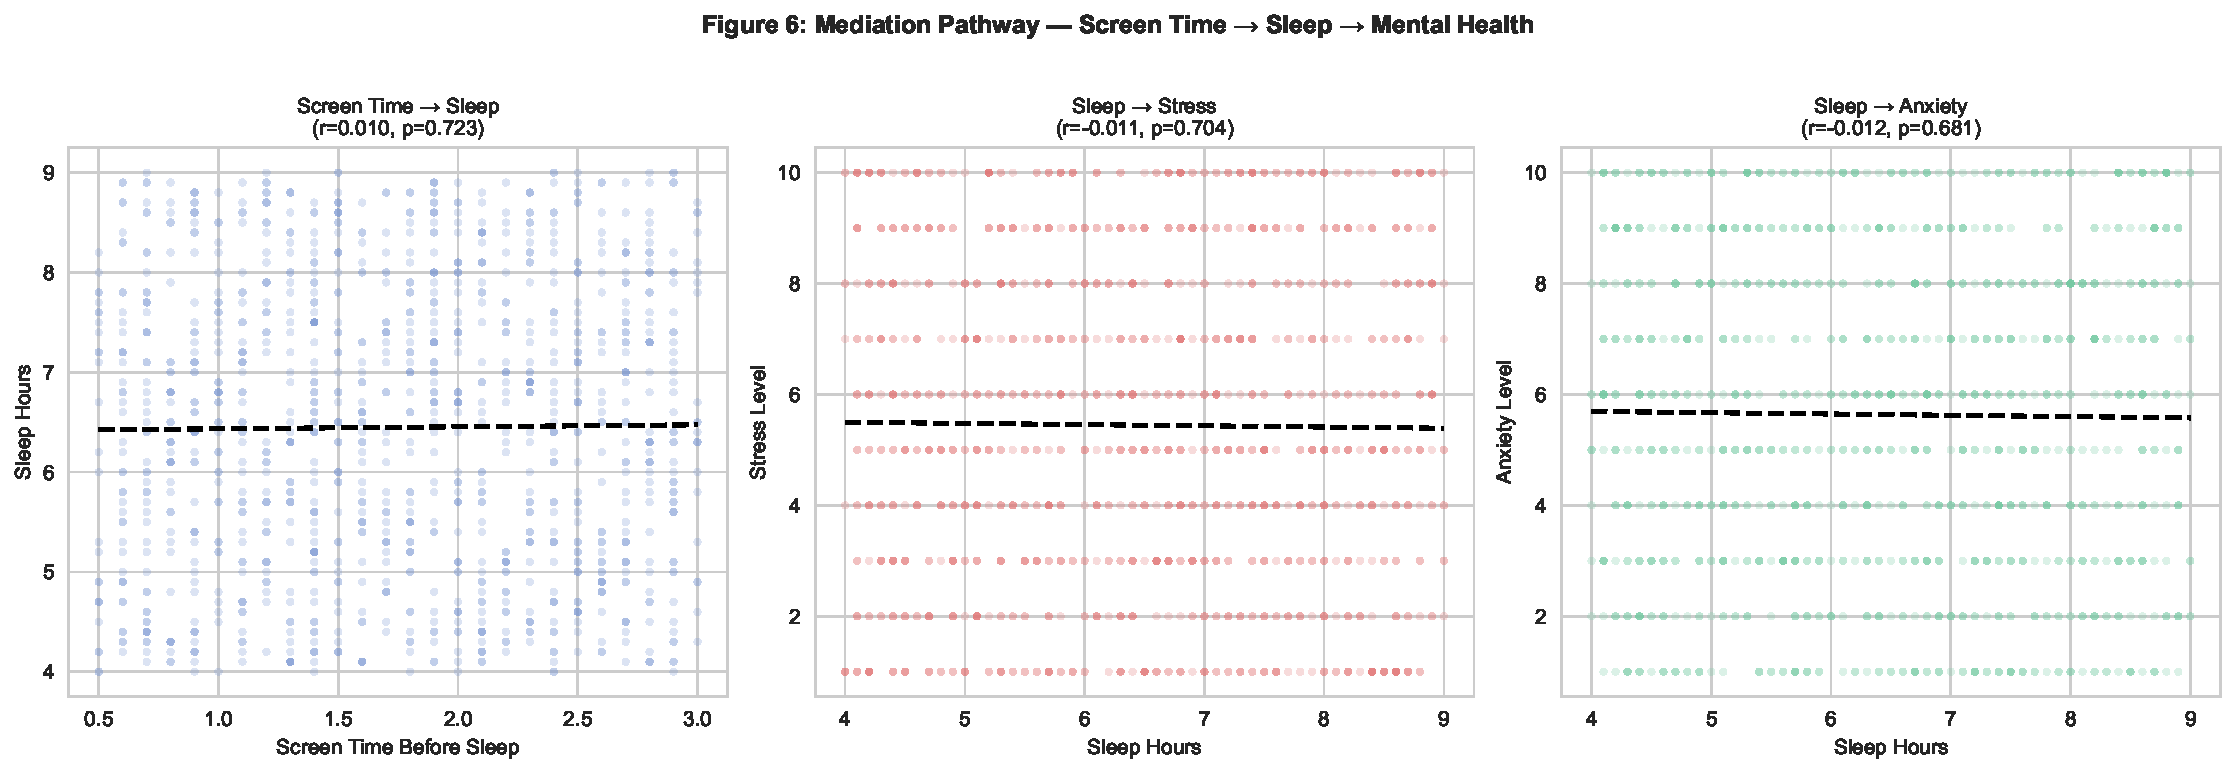
\includegraphics[width=0.95\textwidth]{fig6_mediation_scatter.pdf}
\caption{Mediation pathway scatter plots: (A) pre-sleep screen time vs.\ sleep hours
($r = 0.010$, n.s.); (B) sleep hours vs.\ stress level ($r = -0.011$, n.s.);
(C) sleep hours vs.\ anxiety level ($r = -0.012$, n.s.).  The flat regression lines in
panels (A)--(C) confirm that neither path $a$ nor path $b$ reaches significance, ruling
out formal mediation.}
\label{fig:fig6}
\end{figure}

\begin{figure}[H]
\centering
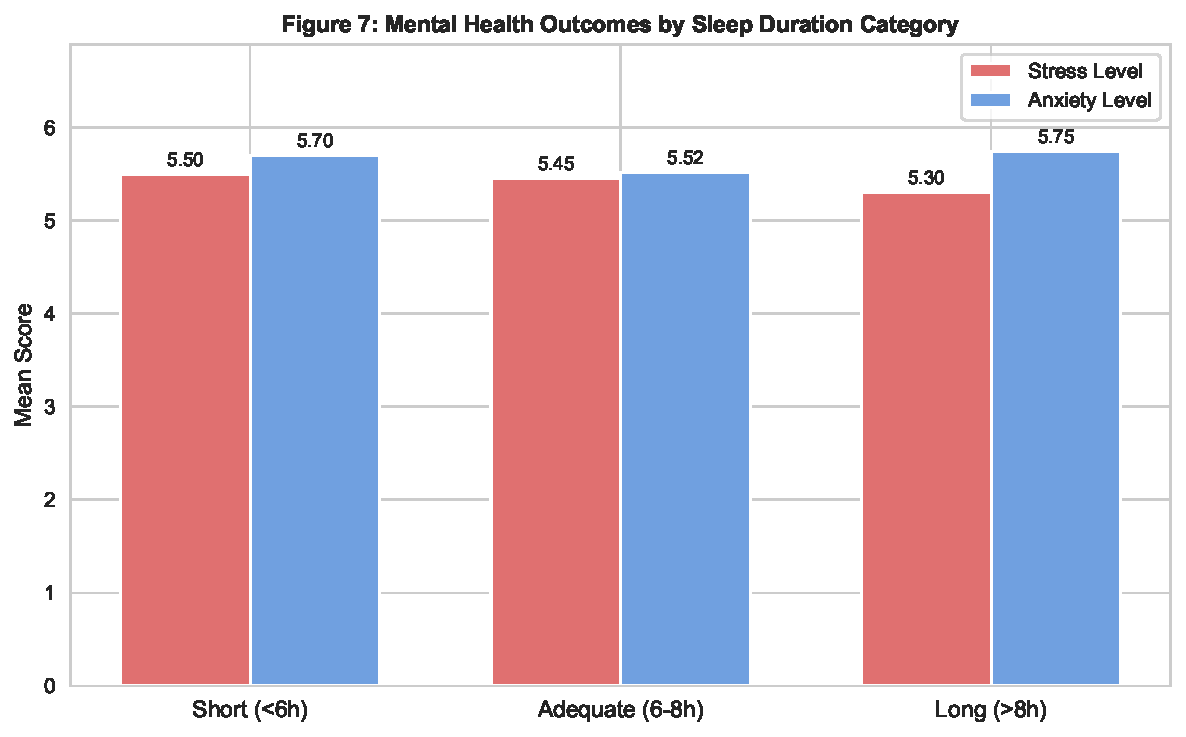
\includegraphics[width=0.75\textwidth]{fig7_sleep_bins.pdf}
\caption{Mean stress and anxiety by sleep duration category. Levels are remarkably stable
across Short, Adequate, and Long sleep groups, consistent with the non-significant mediation
paths. Depression (not shown here) is exclusively concentrated in the Short ($<$6 h) group
(6.5\% vs.\ 0\%), pointing to a threshold rather than graded relationship.}
\label{fig:fig7}
\end{figure}

%%% ─────────────────────────────────────────────────────────
\section{Discussion}
\label{sec:discussion}
%%% ─────────────────────────────────────────────────────────

\subsection{Synthesis of Findings}

Taken together, the three research questions paint a coherent picture.
Sleep deprivation is the single most consequential behavioral factor for adolescent depression,
operating as a threshold rather than as a mediator of other exposures.
The anxiety-stress-social media triad forms a secondary risk cluster.  That social media
\emph{hours} outperform addiction-level scores in the regression model ($\beta = 1.645$
vs.\ $\beta = 0.171$) may reflect measurement issues --- the addiction scale may not
adequately capture problematic usage --- or may genuinely indicate that passive, high-volume
exposure is more detrimental than compulsive short-burst use.

The null dose-response result for RQ2 is notable.  The absence of a linear hourly effect
on stress and anxiety challenges the intuition that ``more screen time = worse mental health,''
at least in cross-sectional data.  Platform type provides a more nuanced story: TikTok's
algorithmically curated short-form video feed appears to be associated with higher anxiety
(particularly at high usage), while multi-platform simultaneous use correlates with higher
stress.

The failure to detect mediation via sleep in RQ3 does not diminish sleep's importance
--- quite the opposite.  The threshold finding (zero depression at $\geq$6 h, 6.5\% at
$<$6 h) suggests that adequate sleep may act as a \emph{moderator} or a \emph{prerequisite}
for resilience rather than as a simple pathway variable.  Future studies should test
this moderation model explicitly.

\subsection{Limitations}

Several limitations warrant caution.

\begin{enumerate}
\item \textbf{Cross-sectional design.}  All three analyses use cross-sectional data, precluding
causal inference.  The observed associations between social media hours and depression may
reflect reverse causality (depressed teens using media to cope).

\item \textbf{Class imbalance.}  With only 31 depression cases (2.6\%), the logistic model
may be overfitting to the majority class despite high AUC.  The impressive accuracy is partly
inflated by the base rate.  A balanced training set or cost-sensitive learning would strengthen
RQ1 conclusions.

\item \textbf{Self-report bias.}  Social media hours, sleep duration, and stress/anxiety levels
are all self-reported, likely introducing recall bias and social desirability effects.

\item \textbf{Platform heterogeneity.}  ``Both'' (multi-platform) is a heterogeneous category
that conflates different usage intensities.  Disaggregating by specific platform combinations
would sharpen the platform moderation analysis.

\item \textbf{Omitted variables.}  Family environment, socioeconomic status, prior mental
health history, and school-related stressors are not included in the dataset and represent
important confounders.
\end{enumerate}

%%% ─────────────────────────────────────────────────────────
\section{Conclusion}
\label{sec:conclusion}
%%% ─────────────────────────────────────────────────────────

This study asked three empirical questions about teen mental health.  The answers are:

\begin{enumerate}
\item \textbf{RQ1 — Best predictors of depression:}  Sleep hours (protective; OR = 0.111),
anxiety (OR = 6.50), stress (OR = 5.68), and daily social media hours (OR = 5.18) jointly
explain adolescent depression risk with near-perfect discrimination (AUC = 0.9936,
McFadden $R^2 = 0.688$).  Sleep deprivation is the single largest modifiable risk factor.

\item \textbf{RQ2 — Social media dose-response:}  No significant linear dose-response exists
between daily social media hours and stress, anxiety, or addiction ($|r| \leq 0.031$,
all $p > 0.06$).  However, platform choice is a meaningful moderator: TikTok users show
the highest anxiety and multi-platform users show the highest stress.

\item \textbf{RQ3 — Sleep as mediator:}  Formal Baron \& Kenny mediation of screen time
effects through sleep is not supported (path $a$: $r = 0.010$, $p = 0.72$).  Nonetheless,
sleeping fewer than 6 hours per night is associated with a 6.5\% depression prevalence
compared with 0\% for adequate sleepers --- a finding with clear public health implications.
\end{enumerate}

From a policy standpoint, interventions that protect adolescent sleep (e.g., delayed school
start times, device curfews, parental guidance on nighttime phone use) hold the greatest
promise for reducing depression risk.  Social media restriction policies may be better
targeted at specific high-anxiety platforms (TikTok) and multi-platform simultaneous use
rather than broad hourly limits.

Future work should employ longitudinal designs, objective sleep actigraphy, and richer
platform-specific engagement metrics to disentangle causality from correlation and to
validate these cross-sectional findings at scale.

%%% ─────────────────────────────────────────────────────────
\section*{Reproducibility}
%%% ─────────────────────────────────────────────────────────

All analyses in this paper are fully reproducible.  The Jupyter notebook
\texttt{research\_notebook.ipynb} (located in the same output directory as this paper)
re-generates all figures and tables from the raw dataset
\texttt{Teen\_Mental\_Health\_Dataset.csv}.  Run:

\begin{verbatim}
jupyter nbconvert --to notebook --execute research_notebook.ipynb \
    --output research_notebook_executed.ipynb
\end{verbatim}

Software versions: Python 3.9+, pandas, scikit-learn, scipy, matplotlib, seaborn.

\end{document}
